\documentclass[11pt,a4paper,twoside]{report}
\usepackage{hyperref}
\usepackage{graphicx}

\newcommand{\Csharp}{%
  {\settoheight{\dimen0}{C}C\kern-.05em \resizebox{!}{\dimen0}{\raisebox{\depth}{\#}}}}

\begin{document}

\tableofcontents

\chapter{How to join the BigARTM project?}
\begin{enumerate}
\item Source code is hosted in a private github repository.
    If you don't have a user on github, please register a free user \href{https://github.com/}{here}.
    Then send the name of your github user to \href{mailto:sashafrey@gmail.com}{sashafrey@gmail.com},
    using ``BigARTM: request access'' in the title of your e-mail.
    In few days you will receive a reply confirming that access had been granted.
\item To clone the repository and build sources, please refer to paragraph
    \hyperref[label:how_to_build]{How to build sources}.
\item Read about the math behind BigARTM library: \\ \url{http://www.machinelearning.ru/wiki/images/2/22/Voron-2013-ptm.pdf}
\item Review the list of open issues: \\
    \url{https://github.com/sashafrey/topicmod/issues?state=open}\\
    Feel free to select some of them which sounds interesting and assign it to yourself.
    To submit you change, follow \hyperref[label:how_to_submit]{How to submit my change} guide.
\item Review the latest discussions here: \\
    \url{https://groups.google.com/forum/#!forum/artm_dev}
\end{enumerate}

\chapter{BigARTM - internal documentation}

\section{Intro}
ToDo: write short gentle introduction that provide links to state of the art articles on topic models and BigARTM.

\paragraph{Main goals for the first release.}
\begin{itemize}
    \item Implementation of core topic modeling algorithms with ARTM (Additive Regularization of Topic Models)
    \item Prefer online algorithms, that do not require storing complete doc-token matrix in memory
    \item Utilize sparsity of doc-token and token-topic matrices
    \item Scale well for 32 CPU cores and higher, efficiently using shared memory within single process
    \item Exhibit high convergence rates
    \item Be portable (written in C/C++, tested with gcc, intel and cl.exe)
    \item Have an interface in Python, Java and $\Csharp$
    \item Be open-source (MIT license)
\end{itemize}
First version we release to public may not have the following features:
\begin{itemize}
    \item Distributed cluster solution
    \item CUDA and Intel Xeon Phi support
\end{itemize}
This is likely to be added in later versions.

\paragraph{Success criteria.}
When codebase meets this success criteria we are free to release the library.
\begin{itemize}
    \item The algorithm scales linearly up to 32 CPU cores when process
    \href{http://archive.ics.uci.edu/ml/datasets/Bag+of+Words}{pubmed task}.
    \item On small datasets perplexity of our method is on parity with other libraries
    \item Builds with gcc, intel and cl.exe compiler; runs on Ubuntu, Solaris and Windows.
    \item No crashes, hangs or memory leaks in stress testing against real-world and model datasets
    \item Convergence rate is well understood
    \item Performance model is well understood (Disk, Memory, CPU)
\end{itemize}

\section{Design}

\subsection{Core components}

Core components are \emph{DataLoader}, \emph{Processor}, and \emph{Merger}.
Interaction between these components is orchestrated by a class called \emph{Instance},
and two queues --- the \emph{processors queue}, and the \emph{merger queue}.
Please, refer to diagrams \ref{fig:diagramm_artm_core} and \ref{fig:diagramm_workflow}.

\begin{figure}[h!]
\begin{centering}
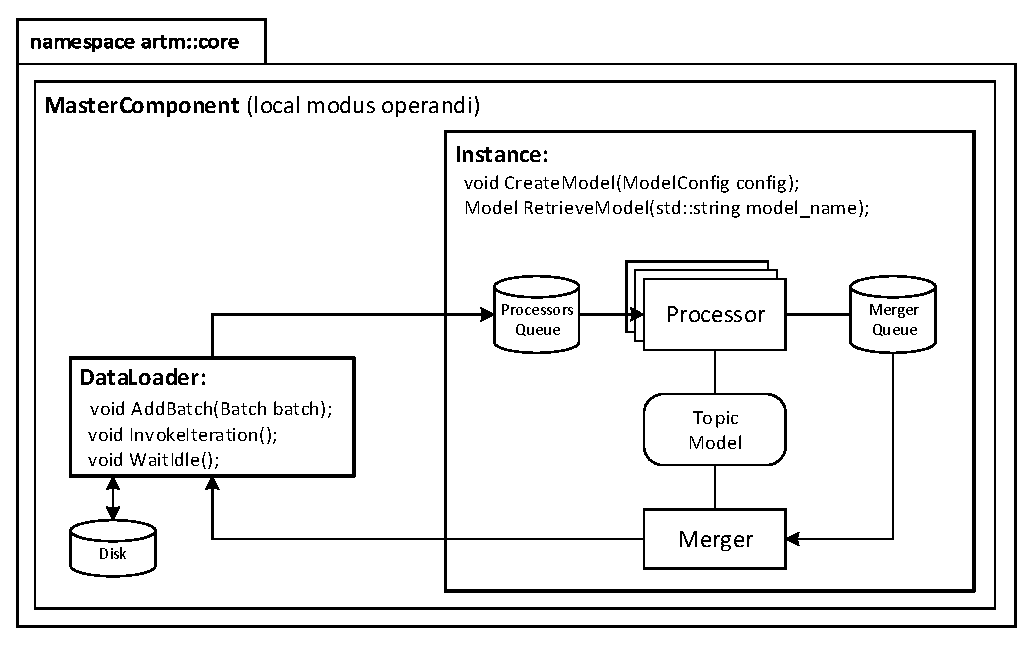
\includegraphics[height=64mm]{diagramm_artm_core.eps}
\caption{Diagram of core ARTM components}
\label{fig:diagramm_artm_core}
\end{centering}
\end{figure}
\vspace{1ex}

\begin{figure}[h!]
\begin{centering}
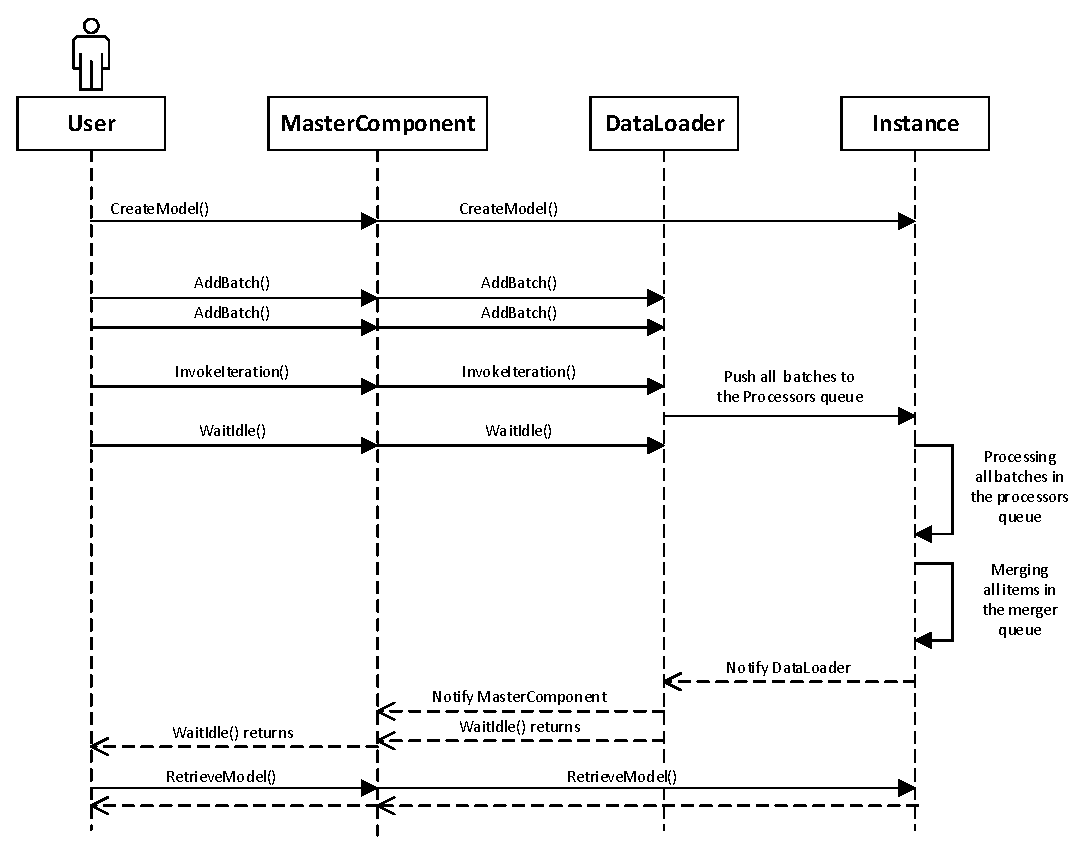
\includegraphics[width=90mm]{diagramm_workflow.eps}
\caption{Interaction between User, DataLoader and Instance}
\label{fig:diagramm_workflow}
\end{centering}
\end{figure}

\textbf{DataLoader.} Responsibility of DataLoader component is to populate the the processors queue
with batches of data (small chunks of the collection).
It is up to implementation of the DataLoader to decide where to gather batches
(they can be stored in memory, on disk, or even came through the network).
DataLoader can be told to trigger a scan over the whole collection,
and then wait for the scan to be finished.

It is possible to set up several \emph{streams} inside DataLoader.
(for example, one stream for training items, and the other for test items).
Models (and quality measures such as perplexity) specify which stream to use for tuning (evaluation).

\textbf{Processor.} Processor component withdraws batches from the processors queue
and infers a distribution of the documents into topics.
The output is stored in \emph{merger queue}.
Before processing a new batch the processor asks merger about the the latest token-topic matrix.

If processor observes a token that is not part of token-token matrix, it stores this token in the list of
new ``discovered'' tokens, and transfers this list as part of processor output.
Merger picks up all such tokens, and initializes new row in token-topic matrix.
So, during the first scan over the collection the dictionary is gathered automatically.

\textbf{Merger.}
Merger reads the merger queue and updates token-topic matrix.
At any moment there exist two copies of token-topic matrix,
an ``active'' and a ``background''.
The ``active'' token-topic matrix is used by processors,
while ``background'' token-topic matrix can be safely updated by merger.
Currently it is merger who automatically decides when to switch ``active''
token-topic matrix to the ``background'' one.
(but ideally user of the library should be able to control this).
Even after switching ``active'' topic-matrix the previous (deprecated) active matrix
will be in use to complete all ongoing processing of batches.
Every new batch will be processed with new matrix.

This design supports multiple concurrent DataLoader, multiple concurrent Processors, but only one Merger.

This design can be extended to cluster environment by implementing a NetworkMerger,
which in addition to merging token-topic matrix within local process should merge it with updates,
coming from NetworkMerger from other nodes.
This design can also utilize CUDA-enabled devices or Index Xeon Phi co-processor
by implementing a special processor (without changing the rest of architecture).
For CUDA the most promising parallelization is to assign CUDA-threads to topic
while inferring a doc-topic distribution.
DataLoader might implement caching, so that if the whole collection fits into memory
it does not have to reload index parts from disk for the second and further scans.

\subsection{API in C++, Python and Java}
Currently the core ARTM functionality is only available from C++,
but it is designed to support Python and Java.

\begin{figure}[h!]
\begin{centering}
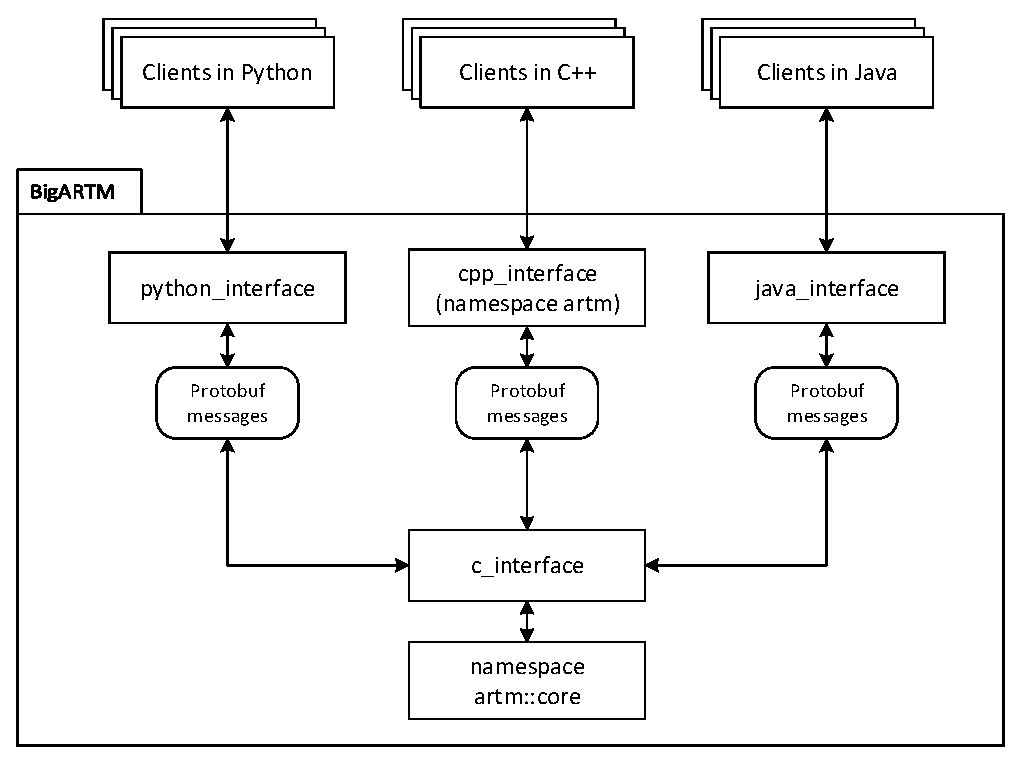
\includegraphics[width=90mm]{diagramm_BigARTM.eps}
\caption{Various interfaces on top of core ARTM components.}
\label{fig:diagramm_BigARTM}
\end{centering}
\end{figure}

\subsection{Concurrency and thread safety}
All interfaces of the library are not thread safe,
and must not be used concurrently from multiple threads.

Internally the library creates multiple threads
(one thread for each DataLoader, Processor and Merger).
Interaction between those threads is synchronized with the following locks:
\begin{enumerate}
    \item Lock access to the processors queue
    \item Lock access to the merger queue
    \item Lock access to the token-topic matrix
\end{enumerate}

We assume that batches are large enough,
and time to transfer a reference from dataloader to processor
is negligible comparing to processing time of one batch.
Access to token-topic matrix is read-only from processor,
so the lock is only needed to retrieve std::shared\_ptr.

DataLoader and Instance components also have their configuration objects,
which can be changed by user of the library during ongoing processing.
For those objects thread-safety is achieved by combining immutable pattern with std::shared\_ptr.
Look at /src/artm/thread\_safe\_holder.h for details.

\subsection{Data layout}
\begin{enumerate}
    \item Doc-token matrix: each doc is represented as list of token ids and their counts
    \item Token-topic matrix: each token is represented the list of topics and their probabilities
    \item Doc-topic matrix: each doc is represented as a sequential vector of topics (no sparsity)
\end{enumerate}

Due to caching in CPU it is important to have topics as a minor dimension in both token-topic and doc-topic matrices.

\subsection{Exceptions and error handling}

\textbf{In c\_interface} all error handling is happening through the error codes.
\begin{verbatim}
  enum ArtmErrorCodes {
    ARTM_SUCCESS = 0,
    ARTM_GENERAL_ERROR = -1,
    ARTM_OBJECT_NOT_FOUND = -2,
    ARTM_INVALID_MESSAGE = -3,
    ARTM_UNSUPPORTED_RECONFIGURATION = -4,
  };
\end{verbatim}  
You are free to add more error types when needed.
The reason for negative values is due to some API methods
returning the actual result; for example, this method returns an ID of newly created object.
\begin{verbatim}
int ArtmCreateDataLoader(int data_loader_id, int length, 
                         const char* config);
\end{verbatim}

\textbf{In artm::core} you should use C++ exceptions 
or simple true/false return values instead of error codes.
Please, follow guidelines in /artm/core/exceptions.h.
Some highlights:
\begin{enumerate}
    \item All exceptions should be inherited for std::runtime\_error
    \item Use BOOST\_THROW\_EXCEPTION macro to throw an exception
    \item Remember to catch all exceptions in c\_interface, and convert them to error codes.
\end{enumerate}

\textbf{In cpp\_interface} all error codes should be converted to exceptions.
Here you should use exceptions, defined in artm/core/cpp\_interface.h file.
Do not re-use existing exceptions from artm::core namespace.

\section{FAQ}

\subsection{What is ``google protocol buffers''}

For an overall introduction about google protocol buffers read the tutorial: \\
\url{https://developers.google.com/protocol-buffers/docs/cpptutorial} \\
Now take a look at file /src/artm/messages.proto,
and the compiled version (other messages.* files).

/src/artm/messages.proto describes the key objects that users can pass into our library.
For example, it defines the following entities:
\begin{itemize}
    \item the representation of a collection of textual files,
    \item all configuration parameters (number of concurrent processors, algorithm to use, etc),
    \item the representation of a topic model which library returns back to the user.
 \end{itemize}

For example, collection is represented as a set of Items.
Items is what you normally call ``documents'' --- they have a list of tokens (aka terms),
together with the number of occurrences of those tokens.
All tokens in each Item are organized into Field (for example, ``body'', ``author'', ``title'', ``year'').
This is a nice way of incorporating metadata into the document.

When passing items into the library those items should be organized into Batches.
Each batch is a collection of items, that share common dictionary of tokens.
Then each items is represented as two vectors --- indexes of tokens in the dictionary,
and the corresponding occurrences.

\paragraph{Key benefits of google protofol buffers}

Once you define you objects in .proto file, you can use them in many programming languages.
Google officially supports C++, Python, and Java. There are also good implementation for $\Csharp$.
I've also heard that it might be something for matlab, but I'm not so sure. Here is how it works:

1. Each proto-message has a serializer, which converts the message into byte array
(and corresponding deserializer that restores an original message).
The clue is that object can be serialized in one language (for example, in Python),
and deserialized in another language (for example, in C++).

2. Passing byte arrays between different languages is very simple.
If you have a .dll (or .so library in Linux) with "extern c" api,
you may call methods in this library from other languages.

As a result, the complex logic of the library can be written once in C++,
and then wrapped into many APIs, as in fig. \ref{fig:diagramm_BigARTM}.

\subsection{There is so much code.. Where should I start?!}

First, take a look at /src/cpp\_client/srcmain.cc.
It is an example of a simple external application build on top of our library ---
it loads a collection of texts from a file,
splits this collections into batches, and sends them into the library.
Then the library tunes a model,
returns it back cpp\_client,
and the client reports top N words in each topic.

Try to run cpp\_client step by step in debugger and see what exactly it does.
To do so you have to unpack all archives under the /datasets folder,
and run cpp\_client with corresponding parameters.
In Linux you may simply use ``make kos'' or ``make nips'' commands.
To run cpp\_client in Windows directly from Visual Studio
you should configure the following command for debugger:

{\small
\begin{verbatim}
$(SolutionDir)..\datasets\docword.kos.txt $(SolutionDir)..\datasets\vocab.kos.txt 16
\end{verbatim}}

\section{Algorithms}

\subsection{Online PLSA}
Online PLSA is the only method implemented at the moment.
It has the following implementation details:
\begin{enumerate}
    \item Processing of documents happens in parallel, according to the design
    \item Strategy of updating matrix $\Phi$: whenever Merger finishes processing of the next Processors output,
    it updates matrix $\Phi$. It will be picked by each processor whenever it starts processing next partition.
    \item Matrix Phi is initialized with random [0..1] values.
    \item By default distributions $\theta_{t d}$ are inferred from scratch on every scan of the collection.
          Processors can be configured to re-use the $\Theta$ values from previous iteration.
    \item Counters $n_{w t}$ and $n_t$ keep increasing, even between scans of the whole collection.
          No exponential decay is currently implemented.
    \item Current perplexity calculation is also cumulative.
          There is stupid limitation: perplexity can't be calculated for a single iteration.
    \item Perplexity can be evaluated on testing items.
          Each item from the testing set is used to both infer theta, and evaluate perplexity.
          An alternative is to randomly split each testing document into two halves.
\end{enumerate}

\section{How to build sources?}
\label{label:how_to_build}

\subsection{Windows}

\begin{enumerate}
   \item Download and install GitHub Windows from \url{http://windows.github.com/}
   \item Clone \url{https://github.com/sashafrey/topicmod/} repository
   \item Download and unpack boost 1.55  \\
         \url{http://sourceforge.net/projects/boost/files/} \\
         Set environmental variable BOOST\_ROOT to the root of our boost installation.
         To do so you may use cmd.exe:
\begin{verbatim}
setx BOOST_ROOT "C:\\Program Files\\boost\\boost_1_55_0"
\end{verbatim}
   \item Download and unpack protobuf 2.5.0 \\
         \url{https://protobuf.googlecode.com/files/protobuf-2.5.0.zip} \\
         Set environmental variable PROTOBUF\_ROOT to the root protocol buffers library.
\begin{verbatim}
setx PROTOBUF_ROOT "C:\\Program Files\\protobuf\\src"
\end{verbatim}
    \item Install Visual Studio 2010 + SP1, or Visual Studio 2012. \\
    {\bf Note: if you use VS2010, you must install Service Pack 1.}
    \item Open /src/artm\_vs2010.sln or /src/artm\_vs2012.sln, depending on your version of Visual Studio.
    \item Build all projects (debug or release, Win32) and execute tests. 64-bit builds are not available yet.
\end{enumerate}

Note: if you got a weird linker error (``error LNK1104: cannot open file 'libprotobuf.lib''')
      in Visual Studio 2010, try this from cmd.exe:
\begin{verbatim}
    setx $(VisualStudioVersion) 10.0
\end{verbatim}
(and then close and reopen Visual Studio, and try clean build).

\subsection{Linux}

\begin{enumerate}
    \item Install git.
    \item git clone https://github.com/sashafrey/topicmod
    \item Install boost (it is preferable to use version 1.55 or newer; \hbox{libboost-all-dev} is package name in Debian-based OS).
    \item Install protobuf (it is necessary to use version 2.5.0 or newer; \hbox{libprotobuf-dev} is package name in Debian-based OS). You can get it from ppa: \hbox{ppa:chris-lea/protobuf}
    \item Use Makefiles under /src/artm/ and /src/cpp\_client/.
\end{enumerate}

\section{How to submit my change to master branch?}
\label{label:how_to_submit}
Every new feature should be developed in a separate git branch.
Usually the integrator (currently \href{mailto:sashafrey@gmail.com}{sashafrey@gmail.com})
merges this feature branches into the master branch.
The key responsibility of the integrator is to ensure stability of the master branch:
\begin{itemize}
    \item No build failures on Windows and on Linux
    \item No new compiler warnings
    \item All unit test passes
    \item Perplexity in cpp\_client looks reasonable
    \item Documentation is updated and compiles in LaTeX
    \item The change passed code review
    \item The change follows our code style
\end{itemize}
Everyone should periodically ``git pull master'' and merge master branch
into their feature branches.

In case if you are absolutely sure you change is safe, feel free to submit the change yourself.
Technically you do have write permissions, so no one can stop you :).
But please do the following:
verify your \hyperref[label:code_style]{code style},
perform \hyperref[label:code_review]{code review},
and make sure everything builds in both Linux and Windows, and unit test passes.

\subsection{Code style}
\label{label:code_style}
In the code we follow
\href{http://google-styleguide.googlecode.com/svn/trunk/cppguide.xml}{google code style},
with the following changes:
\begin{enumerate}
    \item Exceptions are allowed
    \item Indentation must be 2 spaces. Tabs are not allowed.

      If you use Visual Studio,
      please open ``Tools / Text Editor / All languages / Tabs''
      and configure as follows:
      \begin{itemize}
          \item Indenting "--- smart,
          \item Tab size "--- 2,
          \item Indent size "--- 2,
          \item Select "insert spaces".
      \end{itemize}

      We also suggest to show space and tab crlf characters
      in the editor of Visual Studio (shortcut: Ctrl+R, Ctrl+W)

\item No lines should exceed 100 characters.

      If you use Visual Studio, please \href{http://stackoverflow.com/questions/9894397/100-characters-line-marker-in-visual-studio}{enable
       vertical line at 100 characters}.

\item All .h and .cpp files under /src/artm/ must be verified for code style with
      \href{http://google-styleguide.googlecode.com/svn/trunk/cpplint/cpplint.py}{cpplint.py} script.
      It is very easy to use the script; just install
      \href{http://www.python.org/downloads/}{Python 2.7.6}, and run

\begin{verbatim}
python cpplint.py --linelength=100 <filename>
\end{verbatim}
      Files, generated by protobuf compiler, are the only exceptions from this rule.

\item Be careful with C++11 features, and make sure your change builds in Visual Studio 2010.

\end{enumerate}

\subsection{Code review}
\label{label:code_review}
We use
\href{https://code.google.com/p/rietveld/wiki/UploadPyUsage}{rietveld}
tool for code review.
When you have your first change, please learn how to use the
\href{http://codereview.appspot.com/static/upload.py}{unload.py} script.
For example, to upload all changes in between two git revisions you may use this command:
\begin{verbatim}
code review:
python upload.py --server=http://codereview.appspot.com/
 --email=<your_email> -t <review_title> -m <review_description>
 --rev=<from_revision>:<to_revision>
\end{verbatim}
where ``from\_revision'' and ``to\_revision'' may look as follows:
\begin{verbatim}
e26b8107520e219cac89f3cb6ed83b5680240a79
\end{verbatim}

\subsection{Language -- english or russian?}
Feel free to use either English or Russin in all e-mail conversations, including \url{https://groups.google.com/forum/#!forum/artm_dev}.

In the code everything should be in English only, including comments.
It is also preferable to keep this documentation in English.

\end{document}  